
\section{Scheduling}
\label{scheduling}

\subsection{CLP Models for Scheduling}

In time-triggered communications messages are pre-scheduled on the network, and schedule calculation must ensure that messages and their sending and receiving tasks appear at appropriate times in the schedule, as the protocol does not block for message transfers.  For our testing and experimentation we make the following assumptions regarding system models to be scheduled:

\begin{itemize}
\item	All tasks are strictly periodic, or each task is released exactly on a periodic schedule.  
\item	The worst-case execution time (WCET) is known for each task on a given processor.
\item	Tasks assigned to the same processor are not preemptive.
\item	Message buses are shared by multiple processors.
\item	Messages are not strictly periodic (to ease scheduling), but must be delivered on time.
\item	Message transfer times are known.
\item	A feasible bus schedule is not preemptive.
\item Messages are broadcast to all nodes on a bus.
\item On task release input data are already available for use in input buffers. Tasks write output data to output buffers at completion times.  The communication framework transfers data and updates these buffers.
\end{itemize}

All processing nodes execute tasks within the same hyperperiod (repetition window\cite{sched:offline}).  The hyperperiod is the least common multiple of the periods of tasks in the system.  Let $H$ be the hyperperiod length. Each task $T_i$ has maximum duration (WCET) $D_i$ and period $P_i$. Task $T_i$ runs $\frac{H}{{P_i}}$  times during a full cycle of the schedule.  The individual instances (or jobs) of $T_i$ are denoted $T_{i,j}$ where $j \in [1,...\frac{H}{{P_i }}]$.
Task instance $T_{i,j}$ has a start time $R_{i,j}$ which is to be determined.
The same structure is required for messages.  Message $M_i$ has length $E_i$ and instances $M_{i,k}$ having transfer times $S_{i,k}$.

The basic concepts from finite-domain (FD) constraint programming needed for this exposition are covered here in summary only.  A constraint problem is modeled as a set of integer variables and a collection of different types of constraints modeling the relationships between those variables.  Constraints typically include many arithmetic equalities and inequalities. Any valid solution must satisfy all of the constraints. In our case the variables represent the start times of the various task and message instances ($R_{i,j}$ and $S_{i,k}$).  The finiteness of FD constraints refers to the fact that all of these variables are positive and have an explicit upper bound.  Here all variables initially range over the hyperperiod of the schedule.  FD solvers search the solution space by propagating constraints and branching over assignment possibilities.  We use the Gecode finite domain constraint solver library\cite{tools:gecode} within our scheduling tool.

\subsubsection{Task Ordering}

For each task $T_i$ the instances are ordered by the following set of constraints, representing strict periodicity exactly as in \cite{sched:offline}:

\begin{equation}
S_{i,j}  = S_{i,j+1} + D_{i,j}\ \forall j \in [1,...(\frac{H}{{P_i}}-1)]
\end{equation}
	  
For all jobs on the same processor, a global serialization constraint is also imposed to represent non-preemption.  The global serialization constraint forces all variable assignments from the given set to be distinct, and to differ by at least a constant value (duration).  For efficiency (and model conciseness), global distinctness constraints are used instead of $n^2$ constraints representing all possibilities\cite{sched:cumulatives,sched:offline}.  The constant durations are specified for each variable in the constraint, as a pair.  For processor $p$, if $I_p$ is the index set of all task instances on $p$, then we write

\begin{equation}
\forall i \in I_p ,\forall j \in [1,...\frac{H}{{P_i}}]\ ser(R_{i,j}, D_i ).
\end{equation}

Here the function $ser$ represents the global constraint implementation of the set of distinctness constraints.

\subsubsection{Message Ordering}

The existing approach to message ordering constraints in \cite{sched:offline} explicitly represents the relationships between sender and message instances.  To insure that messages were sent between successive sender instances, constraints of the form 

\begin{equation}
R_{i,j}  + D_i  \leqslant S_{l,j}, S_{l,j}  + E_l  \leqslant R_{i,j+1}
\end{equation} 

are used to capture the requirement that each message instance ($M_{l,j}$) begins after its sending task instance ($T_{i,j}$) and ends prior to the start of the next sending task instance ($T_{i,j+1}$).  This captures the logical execution time (LET) constraints as in \cite{modeling:giotto3,timed:let,timed:tdl}. For this description we have assumed that messages and their senders occur at the same rate, so they both types of instances are indexed by $j$.  The resulting ordering can be visualized as in Fig. 3.
%\ref{fig:ordering}.

\begin{figure}
		%[height=50mm,width=50mm]
		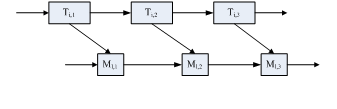
\includegraphics[scale=.6]{figures/ordering.png}
		\centering
	  \label{fig:ordering}
		\caption{Dependency constraints for instances of a message and its sending task.}
\end{figure}

Message instances are all serialized on a given bus, just as for tasks on a processor.  No constraints are imposed on the relationship between message instances and their receivers, as this is handled by latency constraints. We propose the following alternative formulation for message ordering, which is more flexible and at least as efficient for many useful cases. We will first describe the single-rate synchronous case, and then discuss constraints for multi-rate data transfers.

For task $T_i$ sending message $M_l$ (as above), let 

\begin{equation}
\label{eq:msgord}
S_{l,j + 1}  - S_{l,j}  \geqslant P_i  - D_i 
\end{equation}

and

\begin{equation}
\label{eq:wrap}
(H - S_{l,\frac{H}
{{P_i }}} ) + S_{l,1}  \geqslant P_i  - D_i 
\end{equation}

represent the minimum distance between messages as discussed in \cite{sched:constr}.  The second expression (\ref{eq:wrap}) ensures the minimum distance between the last task in the cycle and the first task of the next cycle.
	To ensure the ordering as shown in the diagram we serialize all of the instances of both sender ($R_{i,j}$) and message ($S_{l,j}$) together using a single global serialization constraint:

\begin{equation}
\forall j \in [1,...\frac{H}{{P_i }}],\ ser((R_{i,j} ,D_i ),(S_{l,j} ,E_l ))
\end{equation}

Notice that this approach represents both valid ways of placing the message instances with respect to the senders (see Fig. 4).
%\ref{fig:possibilities}).

\begin{figure}
		%[height=50mm,width=50mm]
		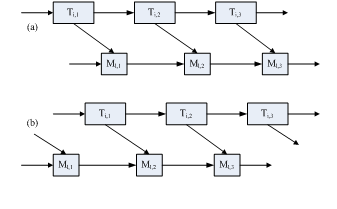
\includegraphics[scale=.6]{figures/possibilities.png}
		\centering
	  \label{fig:possibilities}
		\caption{Two possible valid orderings of constraints for instances of a message and its sending task within one hyperperiod.}
\end{figure}

Handling the multi-rate case requires a small modification to the new constraints.  We assume that the receiver rate is slower than the sender rate (decimation). This is the only case that makes sense, as interpolation could be more efficiently performed by simply keeping and reusing messages on the receiving end.  Suppose $j \in [1,...J]$, $k \in [1,...K]$, and that K divides J (written $K|J$).  This condition is not strictly necessary, but we leave its relaxation as an exercise for the interested reader.  Then we can re-state equations \ref{eq:msgord} and \ref{eq:wrap} as follows to include the decimation term:

\begin{equation}
S_{l,j + 1}  - S_{l,j}  \geqslant (P_i \frac{J}{K} - D_i )
\end{equation}

and

\begin{equation}
(H - S_{l,\frac{H}{{P_i }}} ) + S_{l,1}  \geqslant (P_i \frac{J}{K} - D_i )
\end{equation}

Note that for the simple case $\frac{J}{K} = 2$, this combination of constraints now represents all four possible proper placements of message instances with respect to the sending tasks, greatly increasing the flexibility of the multi-rate scheduling approach presented in \cite{sched:offline}.

\subsubsection{Latency Constraints}

Latency constraints enforce the maximum acceptable response time between the start of a task and the end of a (possibly) different task.  Latencies were originally modeled in \cite{sched:offline} as a disjunctive constraint for handling the possible wrap-around at the end of the message cycle.  The disjunctive constraints apparently created problems for the constraint solver, leading to a two-stage approach to solving the problem \cite{sched:offline}.  In the two-step approach, the solver is run once without the latency constraints to capture a valid ordering of tasks and messages (to break symmetries).  Then the task and message order determined by the solver is used to add the latency constraints.  

Latency modeling is greatly complicated by multi-rate tasks and their dependencies.  An initial ordering capture may lead to an infeasible schedule, without a clear path to backtrack to a different ordering.   Our latency modeling approach does not sacrifice feasibility, but also may not lead to a valid solution.  Implicit in selection of a timing bound for a pair of tasks is the set of chains of dependencies between them.  These could be captured in the model, but path enumeration can easily lead to a combinatorial explosion of paths.  Rather, our approach is to place constraints on the pairs of instances of the starting and ending tasks that try to get them within the specified distance.  Then proper ordering must be checked post-facto (i.e. did all of the intervening tasks and messages occur in the proper order).  Our argument is that this approach could be verified operationally.  For example, re-simulating the control design with the new scheduling order may be a good approach to determine whether time delays introduced by schedule computation have had an effect on the controller requirements.  To converge on a working solution, the designers could iteratively generate a schedule for a given design, simulate the control loops running over that schedule, adjust rate parameters (or make other design changes), and repeat (again refer to \ref{fig:flowchart}).

The latency model is constructed as follows:

\begin{enumerate}
\item Remove redundant constraints -- latency specifications that are larger than the period of either the sending or receiving task.
\item For each remaining latency specification, create $n^2$ reified linear constraints, each requiring that a single sender instance and a single receiver instance fall within the specified time distance.  Reified constraints have an explicit boolean control variable.

\begin{equation}
\label{eq:lat}
(S_{i,k}  - S_{j,l}  \leqslant l_m ) \Leftrightarrow b_n 
\end{equation}

In Eq. \ref{eq:lat} we see sending task instance $T_{i,k}$, receiving task instance $T_{j,l}$, latency bound $l_m$, and boolean control variable $b_n$.

\item Add a constraint on the control variables, so that at least one of the conditions has to be true (Eq. \ref{eq:sum}).

\begin{equation}
\label{eq:sum}
\sum\limits_n {b_n  > 0} 
\end{equation}

\end{enumerate}

The size of the constraint problem for latencies is not ideal, but the final constraint generally ensures that search will be efficient.   Many of the $n^2$ constraints are infeasible or redundant, so the number could be greatly reduced if necessary.  Until this approach introduces significant size or speed issues, we will allow the solver to handle the elimination of redundant and infeasible subsets of those constraints.  Tests to date have not shown any problems (on medium-sized models).

%To increase the generality of the latency constraint we propose the definition of a latency chain.  A latency chain is a sequence of messages (all within a single hyperperiod) whose initial sender, intermediate messages, and final receiver must all occur within a specified time interval.   We assume the instance ordering is already known (as in the two-stage approach mentioned above) and give an example before describing the constraints.
%Let
%
%\begin{equation*}
%T_{1,1}  \to M_{2,1}  \to T_{3,2}  \to M_{3,3}  \to T_{1,3} 
%\end{equation*}
%
%be a task/message sequence. Then for this set of instances we require ordering as shown (via inequality constraints), serialization (of these particular instances), and the total duration sum less than the specified latency.
%
%Consider a serialization of the above example sequence - 
%
%\begin{equation*}
%(R_{1,1} ,3) \to (S_{2,1} ,1) \to (R_{3,2} ,1) \to (S_{3,3} ,4) \to (R_{1,3} ,3)
%\end{equation*}
%
%any latency bound must be more than (or equal to) $3+1+1+4+3 = 12$ and less than a single hyperperiod ($+3$ to account for the length of the starting task).  Any cycles in the latency sequence (here we start and end with $T_1$) must have a latency no more than the hyperperiod (+ length of the repeated task or message).
%	In the language of constraints such a sequence can be modeled as follows:
%
%Consider two sequences of index integers $A = (a_1, a_2,..., a_U)$ and $B = (b_1 ,b_2 ,...,b_U)$
%having odd length (and appropriate range).   $A$ alternately represents the task/message index, and $B$ represents instance indices.  More directly, this is the sequence
%
%\begin{equation}
%T_{a_1,b_1} \to M_{a_2 ,b_2} \to T_{a_3,b_3} \to \ldots \to M_{a_{U-1} ,b_{U-1}} \to T_{a_U ,b_U} 
%\end{equation}
%
%The relevant serialization constraint can be given as
%
%\begin{align*}
%\begin{split}
%&\forall i \in [1,...,\frac{{U-1}}{2}-1], \\
%&ser((R_{a_{2i-1},b_{2i-1}},D_{a_{2i-1}}),(R_{a_U,b_U} ,D_{a_U}),(S_{a_{2i}},D_{a_{2i}}))
%\end{split}
%\end{align*}
%
%The actual latency for the chain is enforced by the constraint
%
%\begin{equation}
%\label{eq:latency}
%(R_{a_U ,b_U }  - R_{a_1 ,b_1 } ) + D_{a_U }  \leqslant latency
%\end{equation}
%
%It may be sufficient to use only the latency bound \ref{eq:latency} as ordering is enforced elsewhere.  This merits some investigation.  Note that the difficulty with latency chains comes when enforcing constraints for multiple chains.  Then intersections of the chains must be taken into account, and the handling of chains that wrap around the end of the cyclic schedule.

\subsection{Specification of Scheduling Problems}


Listing \ref{schedspec} shows an example of a distributed schedule specification with the following elements:

\begin{itemize}
\item {\bf Resolution} (seconds) specifies the size of a single processing tick for the global schedule.  This should correspond to the largest measurable time tick (quantum) of the processors in the network.  All tasks and messages in the schedule timeline are discretized to this resolution.
\item {\bf Proc} specifies a processing node.  Parameters are name, processor speed (Hz), and message send/receive overhead times (these default to zero seconds if unspecified).  Processor names must be unique.
\item {\bf Task} belongs to the most recently specified processor.  A task is characterized by its name, period, and worst-case execution time (WCET) (both in seconds).  We do not address the manner in which the WCET is to be obtained.
\item {\bf Bus} specifies a bus object, characterized by name, transfer speed (bits per second), and transfer overhead (also in seconds).
\item {\bf Msg} includes a name, byte length, sending task, and list of receiving tasks.
\item {\bf Latency} specifies a timing constraint between two tasks in the system.  This could model end-to-end timing constraints between a sensor and an actuator, for example.  The maximum latency is given in seconds.
\end{itemize}

\begin{framed}
%\lstset{basicstyle=\footnotesize,frame=none,label=schedspec,caption=Sample scheduling problem specification.}
\lstset{basicstyle=\small,frame=none,label=schedspec,caption=Scheduling problem specification.}

\begin{lstlisting}
Resolution 2us

Proc P1 100MHz 50us 10us
Task T1 =50Hz 8us
Task T2 =100Hz 10us

Proc P2 100MHz 40us 12us
Task T1 =50Hz 10us
Task T2 =100Hz 10us

Proc P3 100MHz 50us 12us
Task T1 =25Hz 10us
Task T2 =50Hz 5us

Bus B12 1Mb 0us
Msg M1 16B P1/T1 P2/T1

Bus B23 1Mb 0us
Msg M2 2B  P2/T1 P3/T1
Msg M3 4B  P3/T2 P2/T2

Latency 35us P1/T1 P2/T1
% Latency loop
Latency 100us P2/T1 P2/T2
\end{lstlisting}
\end{framed}


Task and message names are unique only within their scope (processor or bus, respectively).  When used globally they are qualified with their scope as shown (e.g. P3/T1). The timing constraints include the various overhead parameters.  For example, once the message length is converted from bytes to time on the bus, we add the transfer overhead to represent the setup time for the particular protocol.  Engineers must measure or estimate platform behavioral parameters and include them in models for the platform.

\subsection{Solution Concerns}

The Gecode FD solver provides pre-programmed branching heuristics (as well as capabilities for building custom branchings).  We branch first on the start time variables (end times are implied), subdividing intervals at the midpoint.  This seems to give a good spacing for tasks and messages in the results.  Latency branching comes second, starting with the maximum latency for each specification.  No effort is made to optimize the schedule to minimize latencies -- the first feasible latency is taken in each case.  

\subsection{Limitations}

ESched has a number of limitations:

\begin{itemize}
\item We do not support mode switching.  For specification languages that allow mode switching only at the end of the hyperperiod, individual modes can be formulated as separate schedule problems.  Finer-grained switching is not supported.
\item Time-triggered hardware protocols such as TTP/C or FlexRay subdivide hyperperiods into fixed-length slots and limit message transfers to ease schedule calculation.  Compatibility with these protocols would require additional constraints to model the starting and ending times of the slots as well as communication limits (e.g., limiting a task to send a message only once per slot).
\item The overhead parameters may be an overly simplistic model for some cases.  Each processor and bus pair may have different parameters, depending on the bus type and the protocol used.
The scheduling model is discretized to a single resolution for everything in the system.  In reality different processors and buses have different timing characteristics.  We also do not account for uncertainty due to time synchronization, though it could be included in the overhead parameters.
\end{itemize}
